% =============================================================
% 8 Анализ динамики роторной системы на подшипниках скольжения
%   с микроструктурами поверхности
% =============================================================
\chapter{Анализ динамики роторной системы на подшипниках скольжения с микроструктурами поверхности}

\section{Объект исследования и постановка задачи}

В главах~5 и~6 исследовалась стационарная несущая способность
радиального подшипника скольжения при наличии детерминированных
микроструктур рабочей поверхности. Настоящая глава посвящена
анализу динамического поведения системы «ротор~-- подшипник»
при наличии детерминированных микроструктур рабочей поверхности~\cite{miraskari2018a,miraskari2018b,muszynska1988}.
Исследуется тот же радиальный подшипник насоса (глава~5):
$R = 35$~мм, $c = 50$~мкм, $L = 56$~мм, $n = 2980$~об/мин.

Цель~-- оценить влияние текстуры~T2 (конфигурация с наилучшими
статическими характеристиками по результатам главы~5)
на коэффициенты динамической жёсткости, демпфирования, линейную
устойчивость и характер движения ротора в сравнении с гладким
подшипником~\cite{goodwin1997,jang1999,sayed2022}. Анализ выполнен в линейном приближении; основные выводы
формулируются для диапазона $\varepsilon = 0{,}2$--$0{,}6$.
Точка $\varepsilon = 0{,}8$ приводится на рисунках как
дополнительное качественное наблюдение.

Основные параметры модели сведены в таблицу~\ref{tab:dyn_params}.

\begin{table}[!ht]
\centering
\caption{Параметры динамической модели системы «ротор~-- подшипник»}
\label{tab:dyn_params}
\begin{tabularx}{\textwidth}{|X|c|c|c|}
\hline
\multicolumn{1}{|c|}{\textbf{Параметр}} & \textbf{Обозначение} & \textbf{Значение} & \textbf{Единица} \\
\hline
Радиус цапфы            & $R$        & 35{,}0   & мм \\
\hline
Длина подшипника        & $L$        & 56{,}0   & мм \\
\hline
Радиальный зазор        & $c$        & 50       & мкм \\
\hline
Динамическая вязкость   & $\mu$      & 0{,}01105 & Па$\cdot$с \\
\hline
Частота вращения        & $n$        & 2980     & об/мин \\
\hline
Угловая скорость        & $\omega$   & 311{,}9  & рад/с \\
\hline
Масса ротора            & $m$        & 10{,}0   & кг \\
\hline
Масса дисбаланса        & $m_u$      & 1{,}0    & г \\
\hline
Эксцентриситет дисбаланса & $e_u$    & 1{,}0    & мм \\
\hline
Диапазон $\varepsilon$  & --         & 0{,}2--0{,}6 & -- \\
\hline
\end{tabularx}
\end{table}


\section{Расчётная схема и принятые допущения}

Расчёт выполняется в системе координат $x$, $y$, связанной
с подшипником; ось~$x$ направлена по внешней нагрузке. Функция
смазочного зазора:
\begin{equation}
  h(\varphi, z, t) = c + x(t)\cos\varphi + y(t)\sin\varphi
    + h_{\mathrm{tex}}(\varphi, z).
  \label{eq:dyn_h}
\end{equation}
Данное выражение является единым для всех расчётов~-- статики,
динамики, вычисления сил и коэффициентов. Слагаемое
$h_{\mathrm{tex}}$ описывает эллипсоидальные лунки
конфигурации~T2 (подраздел~5.4).

Рабочая точка $(x_0,\, y_0)$ задаётся параметрически через
эксцентриситет: $x_0 = \varepsilon c$, $y_0 = 0$. Поиск
равновесия из уравнения баланса сил в данной главе не
выполняется; малые возмущения $\xi(t)$, $\eta(t)$
рассматриваются относительно заданной точки.

Модель принята изотермической ($T = T_0$,
$\mu = \mathrm{const}$); нелинейное нестационарное
пересчитывание поля давления на каждом шаге не выполняется.
Анализ ограничен линейной моделью малых возмущений.


\section{Математическая модель динамического смазочного слоя}

\textit{Статическое уравнение Рейнольдса.}
Безразмерная форма стационарного уравнения Рейнольдса
(глава~2, формула~\eqref{eq:reynolds_nondim}) для радиального
подшипника записывается в виде:
\begin{equation}
  \frac{\partial}{\partial\varphi}\!\left[H^3\,
    \frac{\partial P}{\partial\varphi}\right]
  + \left(\frac{R}{L}\right)^{\!2}
    \frac{\partial}{\partial Z}\!\left[H^3\,
    \frac{\partial P}{\partial Z}\right]
  = \frac{\partial H}{\partial\varphi}.
  \label{eq:dyn_reynolds_stat}
\end{equation}

\textit{Динамическое уравнение Рейнольдса.}
При учёте движения цапфы к правой части добавляется член сжатия
(squeeze-term), обусловленный производной зазора по времени:
\begin{equation}
  \frac{\partial}{\partial\varphi}\!\left[H^3\,
    \frac{\partial P}{\partial\varphi}\right]
  + \left(\frac{R}{L}\right)^{\!2}
    \frac{\partial}{\partial Z}\!\left[H^3\,
    \frac{\partial P}{\partial Z}\right]
  = \frac{\partial H}{\partial\varphi}
    + \frac{2R}{U}\,\frac{\partial H}{\partial t}.
  \label{eq:dyn_reynolds_dyn}
\end{equation}
Производная зазора по времени выводится из функции
зазора~\eqref{eq:dyn_h}:
\begin{equation}
  \frac{\partial h}{\partial t}
    = \dot{x}\cos\varphi + \dot{y}\sin\varphi.
  \label{eq:dyn_squeeze}
\end{equation}
Никаких дополнительных слагаемых, кроме следующих
из~\eqref{eq:dyn_h}, не вводится.

Граничные условия: периодичность по~$\varphi$; $P = 0$ при
$Z = \pm 1$; $P \geq 0$ (кавитация по условию Рейнольдса).

\textit{Гидродинамические силы.}
Компоненты силы, действующей на цапфу со стороны смазочного слоя,
вычисляются интегрированием поля давления:
\begin{align}
  F_x &= -\iint P\cos\varphi\,\mathrm{d}\varphi\,\mathrm{d}Z
    \cdot F_{\mathrm{scale}},
  \label{eq:dyn_Fx} \\
  F_y &= -\iint P\sin\varphi\,\mathrm{d}\varphi\,\mathrm{d}Z
    \cdot F_{\mathrm{scale}},
  \label{eq:dyn_Fy}
\end{align}
где $F_{\mathrm{scale}} = p_0 R L / 2$,\;
$p_0 = 6\mu U R / c^2$.

\textit{Коэффициенты жёсткости и демпфирования.}
Коэффициенты линейной модели определяются через частные
производные сил по координатам и скоростям:
\begin{equation}
  K_{xx} = -\frac{\partial F_x}{\partial x},\quad
  K_{xy} = -\frac{\partial F_x}{\partial y},\quad
  K_{yx} = -\frac{\partial F_y}{\partial x},\quad
  K_{yy} = -\frac{\partial F_y}{\partial y},
  \label{eq:dyn_K}
\end{equation}
\begin{equation}
  C_{xx} = -\frac{\partial F_x}{\partial\dot{x}},\quad
  C_{xy} = -\frac{\partial F_x}{\partial\dot{y}},\quad
  C_{yx} = -\frac{\partial F_y}{\partial\dot{x}},\quad
  C_{yy} = -\frac{\partial F_y}{\partial\dot{y}}.
  \label{eq:dyn_C}
\end{equation}
Жёсткости вычисляются через статический solver,
демпфирование~-- через динамический solver. Все производные~--
вокруг одной и той же точки $(x_0,\, y_0)$. Ручная коррекция
знаков не применяется.

\textit{Модель ротора.}
Уравнения движения для малых возмущений
$\xi = x - x_0$, $\eta = y - y_0$:
\begin{align}
  m\ddot{\xi} + C_{xx}\dot{\xi} + C_{xy}\dot{\eta}
    + K_{xx}\xi + K_{xy}\eta &= F_{x,\mathrm{unb}}(t),
  \label{eq:dyn_ode_x} \\
  m\ddot{\eta} + C_{yx}\dot{\xi} + C_{yy}\dot{\eta}
    + K_{yx}\xi + K_{yy}\eta &= F_{y,\mathrm{unb}}(t).
  \label{eq:dyn_ode_y}
\end{align}
Сила дисбаланса:
\begin{equation}
  F_{x,\mathrm{unb}} = m_u e_u \omega^2 \cos(\omega t),\qquad
  F_{y,\mathrm{unb}} = m_u e_u \omega^2 \sin(\omega t).
  \label{eq:dyn_unbalance}
\end{equation}

Критерий устойчивости~-- максимальная вещественная часть
собственных значений матрицы состояния системы $4 \times 4$:
$\mathrm{Re}(\lambda_{\max}) < 0$~-- система устойчива.


\section{Численная реализация и верификация модели}

Расчётная область дискретизируется равномерной сеткой
$360 \times 120$ узлов по~$\varphi$ и~$Z$ (точка~$2\pi$
не дублируется). Статический solver~-- пакет
\texttt{reynolds\_solver} (глава~5); динамический solver
реализован отдельно с идентичной дискретизацией и добавленным
squeeze-term. Оба решателя используют метод SOR
с~$\omega_{\mathrm{SOR}} = 1{,}5$,
$\mathrm{TOL} = 10^{-5}$. Коэффициенты вычисляются
центральными разностями с шагами $\Delta x = 0{,}005c$,
$\Delta v = 0{,}005U$.

Для проверки численной устойчивости выполнены два контрольных
расчёта при $\varepsilon = 0{,}6$: шаг конечных разностей
уменьшен вдвое ($\Delta x \to \Delta x/2$,
$\Delta v \to \Delta v/2$) и сетка увеличена до
$480 \times 160$. Результаты верификации для гладкого подшипника как базового
варианта сведены в таблицу~\ref{tab:dyn_verif}.

\begin{table}[!ht]
\centering
\caption{Верификация численной устойчивости при $\varepsilon = 0{,}6$
  (гладкий подшипник)}
\label{tab:dyn_verif}
\small
\begin{tabular}{|l|c|c|c|c|}
\hline
\textbf{Показатель}
  & $\mathbf{360 \times 120}$\textbf{,}
  & $\mathbf{360 \times 120}$\textbf{,}
  & $\mathbf{480 \times 160}$\textbf{,}
  & \textbf{Откл. при} \\
  & $\boldsymbol{\Delta x{,}\,\Delta v}$\textbf{ ном.}
  & $\boldsymbol{\Delta x/2{,}\,\Delta v/2}$
  & $\boldsymbol{\Delta x{,}\,\Delta v}$\textbf{ ном.}
  & \textbf{сгущении сетки} \\
\hline
$K_{xx}$, $10^8$~Н/м & $3{,}51$ & $3{,}51$ & $3{,}52$ & 0{,}4 \\
\hline
$K_{yy}$, $10^8$~Н/м & $1{,}20$ & $1{,}20$ & $1{,}20$ & 0{,}0 \\
\hline
$K_{xy}$, $10^8$~Н/м & $1{,}26$ & $1{,}26$ & $1{,}26$ & 0{,}1 \\
\hline
$K_{yx}$, $10^8$~Н/м & $-1{,}84$ & $-1{,}84$ & $-1{,}85$ & 0{,}6 \\
\hline
$C_{xx}$, $10^6$~Н$\cdot$с/м & $2{,}57$ & $2{,}57$ & $2{,}57$ & 0{,}0 \\
\hline
$C_{yy}$, $10^6$~Н$\cdot$с/м & $1{,}08$ & $1{,}08$ & $1{,}08$ & 0{,}0 \\
\hline
$\mathrm{Re}_{\max}$ & $-122{,}3$ & $-121{,}7$ & $-122{,}6$ & $|\Delta| = 0{,}2$ \\
\hline
\end{tabular}
\end{table}

\FloatBarrier

Верификационные расчёты для гладкого подшипника при
$\varepsilon = 0{,}6$ показали, что коэффициенты жёсткости
$K_{ij}$ и прямые коэффициенты демпфирования $C_{xx}$, $C_{yy}$
слабо зависят от уменьшения шага конечного дифференцирования
и от сгущения сетки (отклонение менее~$1\,\%$). Для
текстурированного варианта~T2 в области больших эксцентриситетов
наблюдается более высокая чувствительность отдельных коэффициентов
жёсткости к разрешению сетки; однако качественные выводы о влиянии
текстуры сохраняются.
Перекрёстные коэффициенты демпфирования $C_{xy}$, $C_{yx}$
проявляют повышенную чувствительность к шагу $\Delta v$
и не используются в данной работе как количественный результат.


\section{Влияние эксцентриситета на коэффициенты жёсткости}

Прямые коэффициенты жёсткости $K_{xx}$ и $K_{yy}$ монотонно
возрастают с ростом~$\varepsilon$ для обоих вариантов
(рисунок~\ref{fig:dyn_K_direct}). На рисунках для полноты
сопоставления дополнительно приведена точка
$\varepsilon = 0{,}8$; основные количественные выводы настоящей
главы относятся к диапазону
$\varepsilon = 0{,}2$--$0{,}6$. Конфигурация~T2 обеспечивает
существенно более высокие значения $K_{xx}$ по всему диапазону:
при $\varepsilon = 0{,}6$ значение
$K_{xx}^{(T2)} = 6{,}25 \cdot 10^8$~Н/м против
$K_{xx}^{(\text{гл.})} = 3{,}51 \cdot 10^8$~Н/м, то есть
прирост составляет около~$78\,\%$. Коэффициент $K_{yy}$ у~T2
также выше и при $\varepsilon = 0{,}6$ составляет
$2{,}06 \cdot 10^8$~Н/м против $1{,}20 \cdot 10^8$~Н/м.

Перекрёстные коэффициенты $K_{xy} > 0$ и $K_{yx} < 0$
сохраняют свои знаки во всём основном диапазоне
$\varepsilon = 0{,}2$--$0{,}6$ для обоих вариантов
(рисунок~\ref{fig:dyn_K_cross}). Их значения для гладкого
и текстурированного подшипников сопоставимы по порядку величины;
конфигурация~T2 не приводит к принципиальному изменению характера
перекрёстной жёсткостной связи.

Сводные значения коэффициентов при $\varepsilon = 0{,}6$
приведены в таблице~\ref{tab:dyn_coeffs}.

\begin{table}[!ht]
\centering
\caption{Коэффициенты жёсткости, демпфирования и запас
  устойчивости при $\varepsilon = 0{,}6$}
\label{tab:dyn_coeffs}
\small
\begin{tabular}{|l|c|c|c|c|c|c|c|}
\hline
\textbf{Вариант}
  & $\boldsymbol{K_{xx}}$, & $\boldsymbol{K_{yy}}$,
  & $\boldsymbol{K_{xy}}$, & $\boldsymbol{K_{yx}}$,
  & $\boldsymbol{C_{xx}}$, & $\boldsymbol{C_{yy}}$,
  & $\boldsymbol{\mathrm{Re}_{\max}}$ \\
  & $10^8$~Н/м & $10^8$~Н/м
  & $10^8$~Н/м & $10^8$~Н/м
  & $10^6$~Н$\cdot$с/м & $10^6$~Н$\cdot$с/м
  & \\
\hline
Гладкий
  & $3{,}51$ & $1{,}20$ & $1{,}26$ & $-1{,}84$
  & $2{,}57$ & $1{,}08$
  & $-122{,}3$ \\
\hline
T2
  & $6{,}25$ & $2{,}06$ & $1{,}23$ & $-1{,}76$
  & $1{,}85$ & $0{,}90$
  & $-282{,}5$ \\
\hline
\end{tabular}
\end{table}

\FloatBarrier

Значение $\varepsilon = 0{,}6$ выбрано как характерный режим
с выраженным динамическим эффектом текстурирования. Для
конфигурации~T2 в данной точке наблюдается умеренная
чувствительность прямых коэффициентов жёсткости к разрешению
сетки, не меняющая качественных выводов.

\begin{figure}[!ht]
\centering
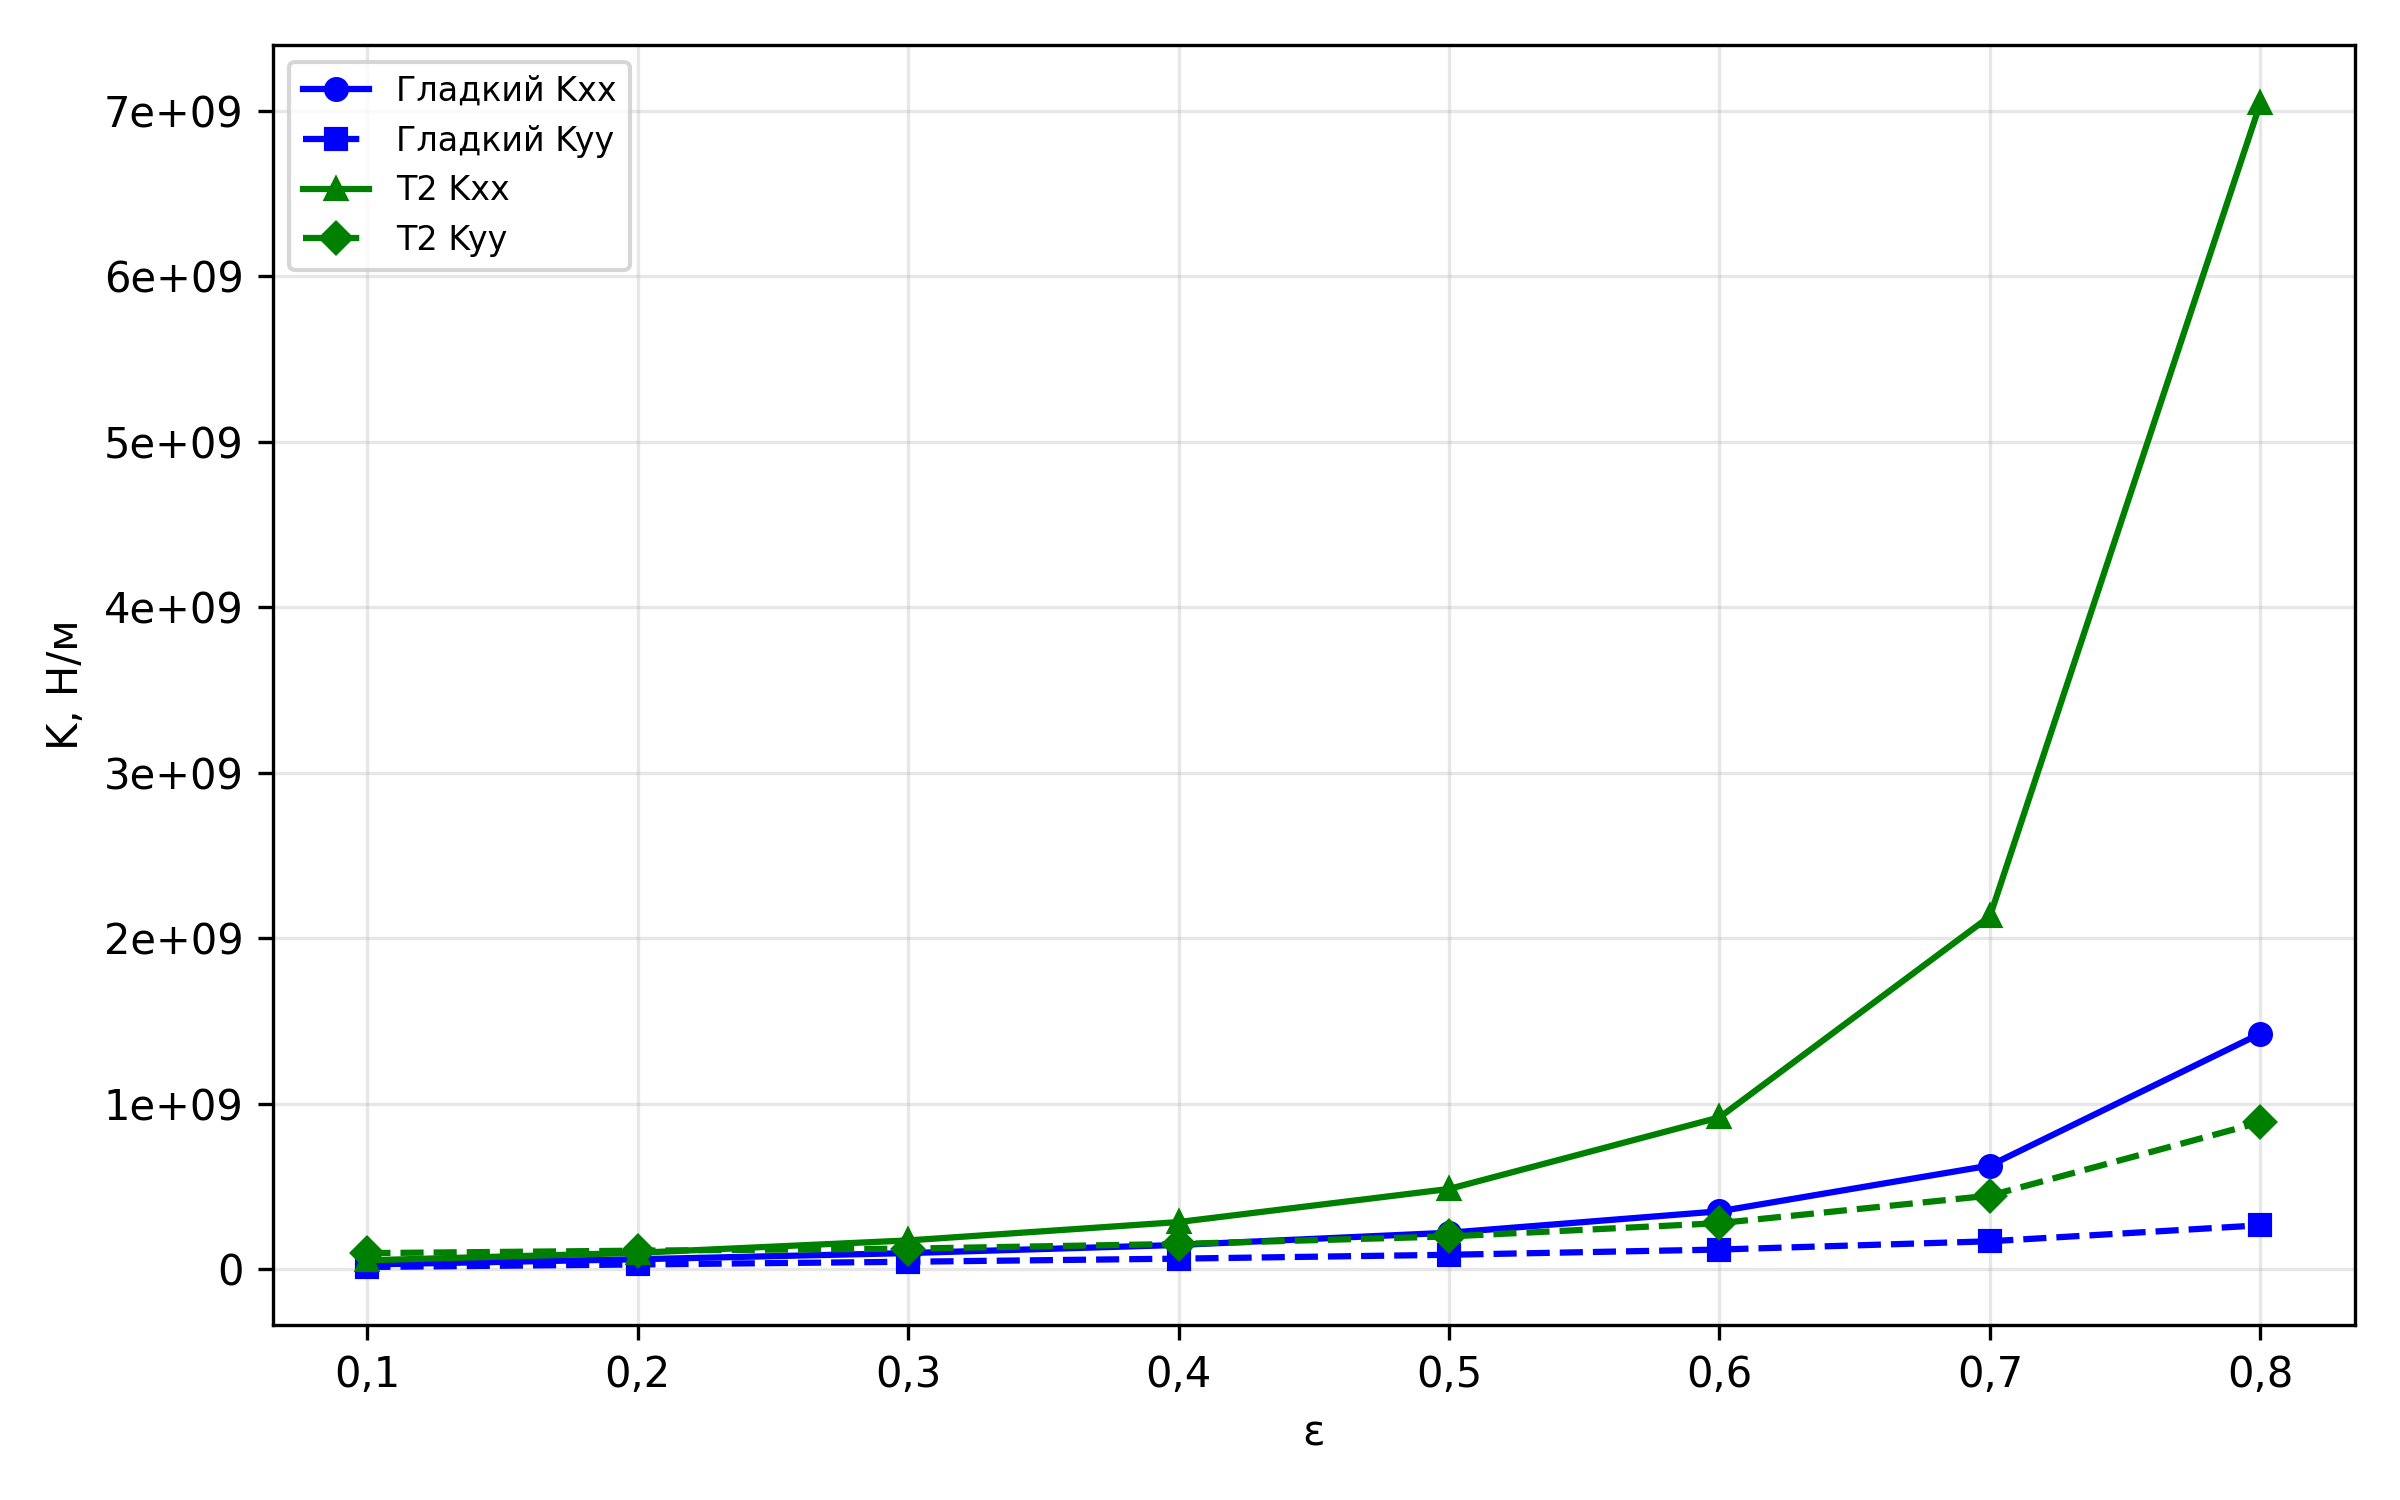
\includegraphics[width=\textwidth,height=0.9\textheight,keepaspectratio]{figures/ch08/fig_8_1.png}
\caption{Зависимость прямых коэффициентов жёсткости $K_{xx}$ и $K_{yy}$
  от относительного эксцентриситета~$\varepsilon$
  для гладкого подшипника и конфигурации~T2.}
\label{fig:dyn_K_direct}
\end{figure}

\begin{figure}[!ht]
\centering
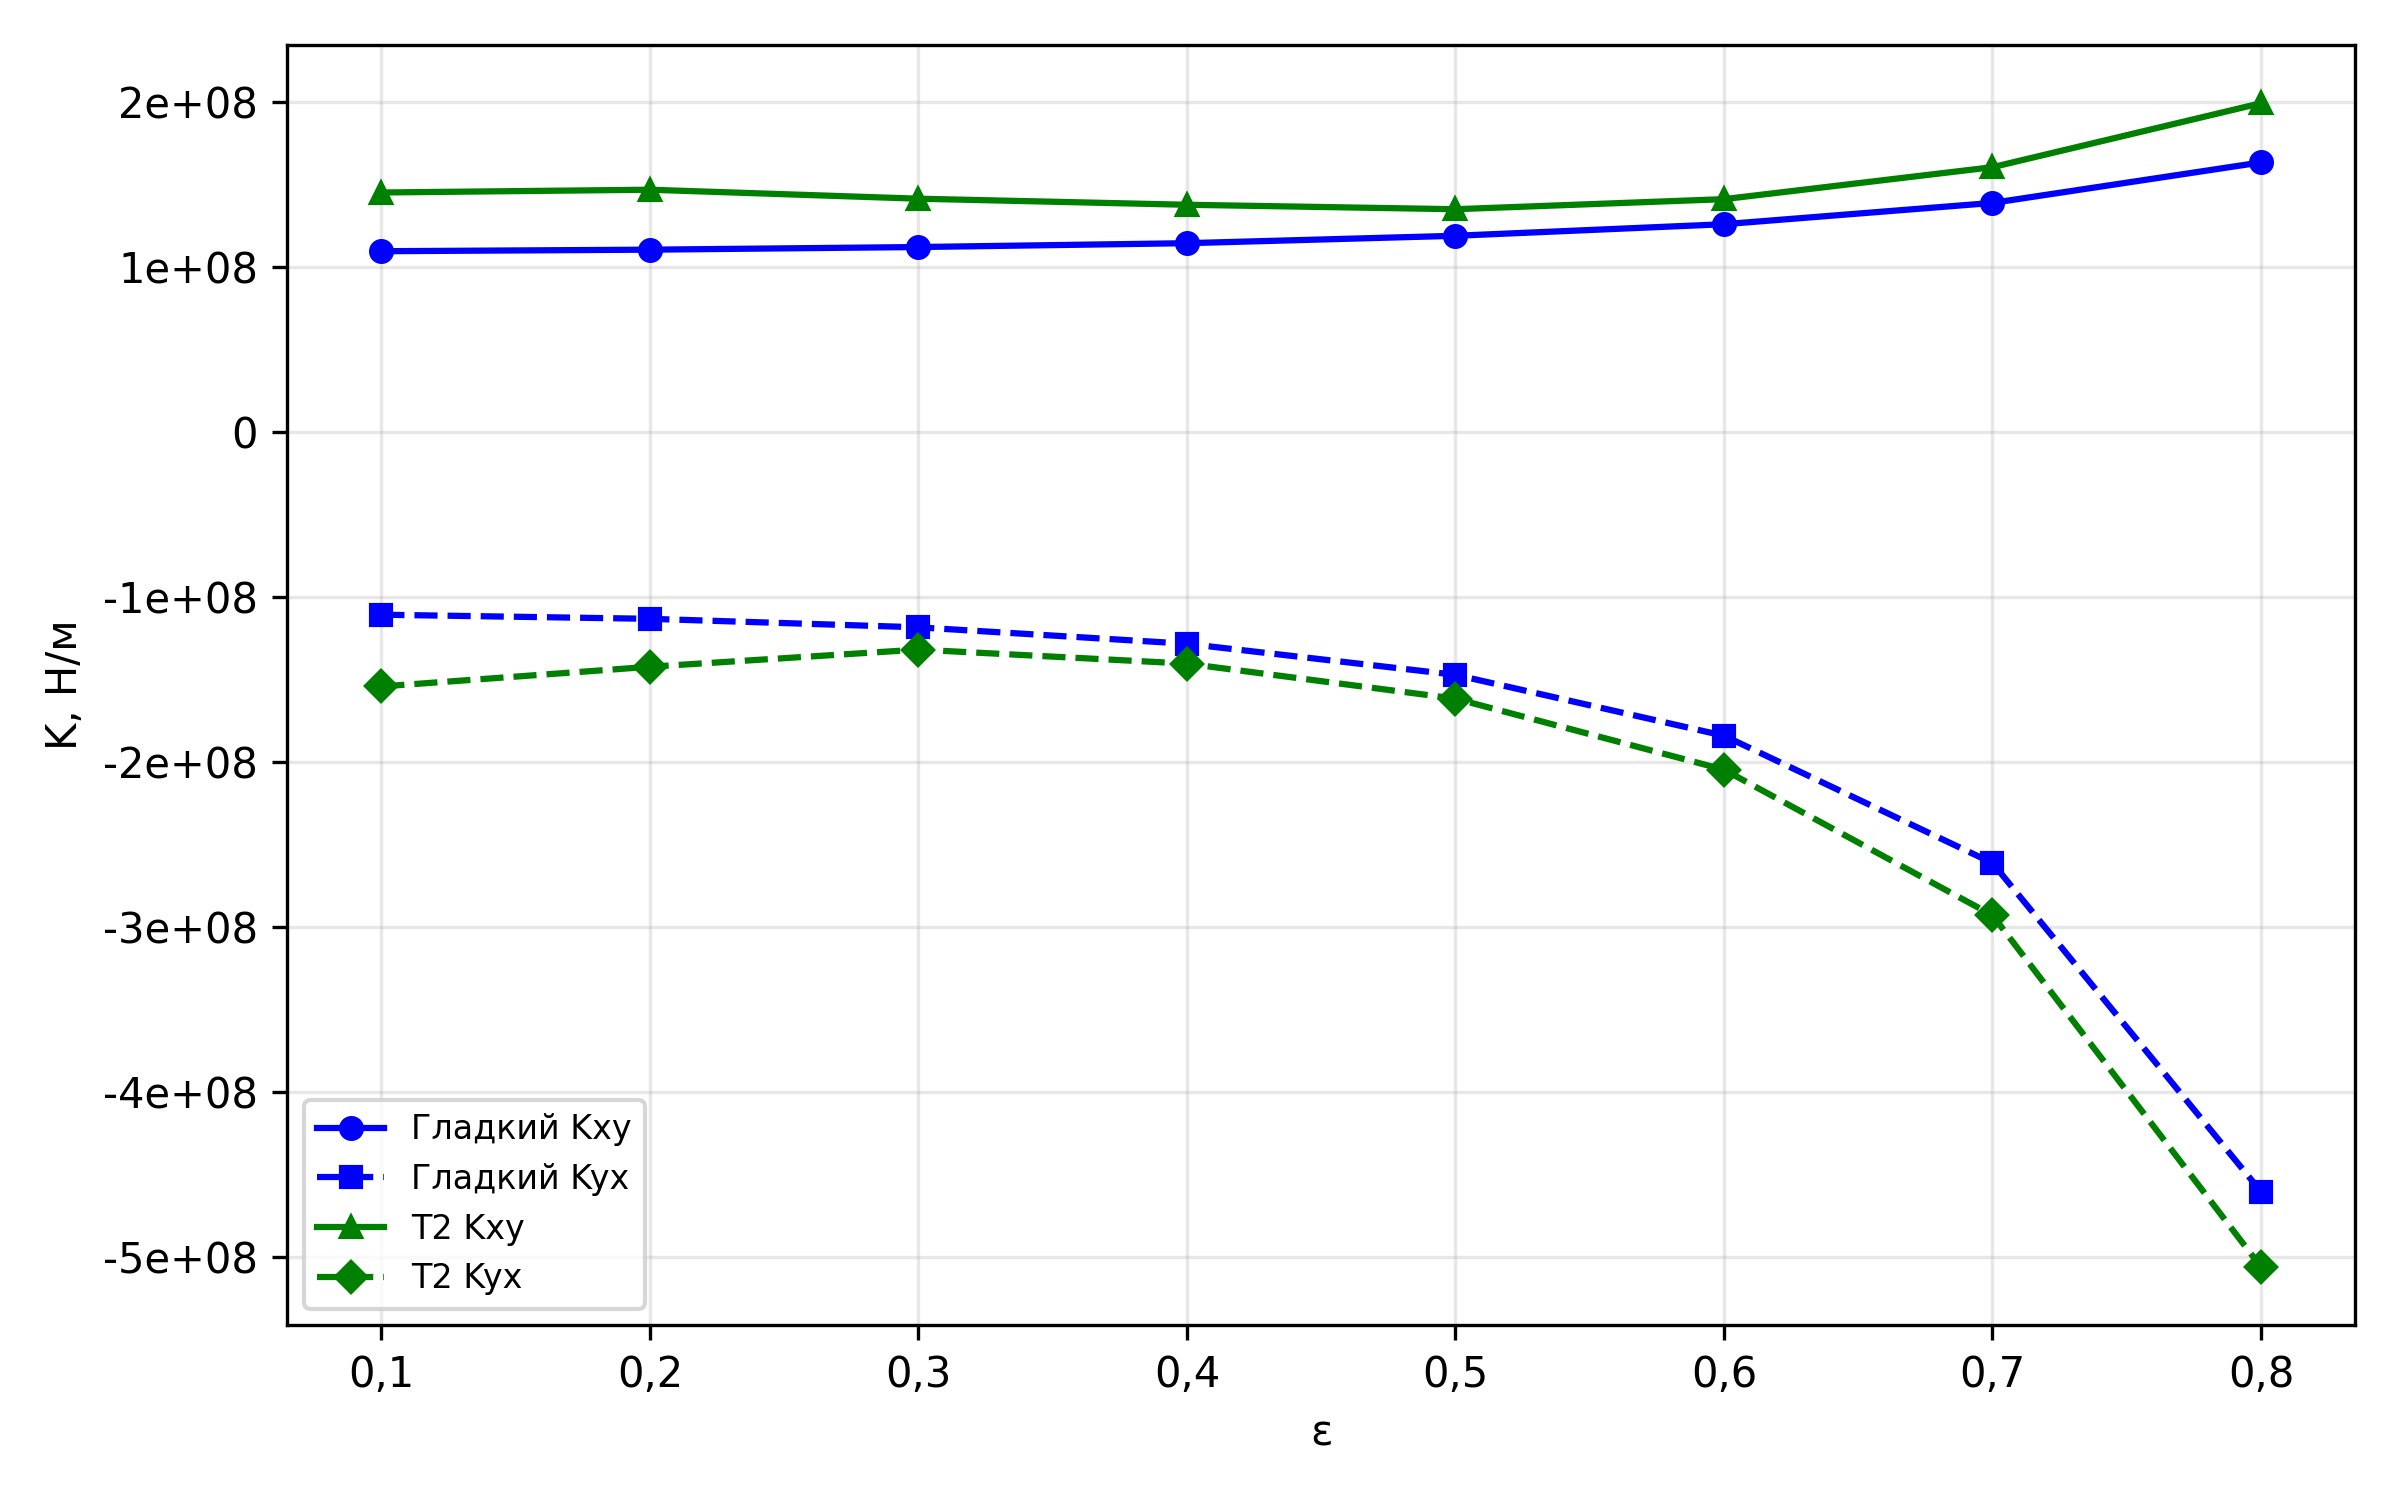
\includegraphics[width=\textwidth,height=0.9\textheight,keepaspectratio]{figures/ch08/fig_8_2.png}
\caption{Зависимость перекрёстных коэффициентов жёсткости $K_{xy}$
  и $K_{yx}$ от эксцентриситета~$\varepsilon$.}
\label{fig:dyn_K_cross}
\end{figure}


\section{Влияние эксцентриситета на коэффициенты демпфирования}

Прямые коэффициенты демпфирования $C_{xx}$ и $C_{yy}$ монотонно
возрастают с ростом~$\varepsilon$
(рисунок~\ref{fig:dyn_C_direct}). Конфигурация~T2 демонстрирует
несколько меньшие значения $C_{xx}$ и $C_{yy}$ по сравнению
с гладким подшипником. При $\varepsilon = 0{,}6$:
$C_{xx}^{(T2)} = 1{,}85 \cdot 10^6$~Н$\cdot$с/м против
$C_{xx}^{(\text{гл.})} = 2{,}57 \cdot 10^6$~Н$\cdot$с/м.

Перекрёстные коэффициенты демпфирования $C_{xy}$, $C_{yx}$
получены как предварительные оценки. Вследствие повышенной
чувствительности к шагу $\Delta v$ они не используются в данной
работе в качестве основных количественных показателей и не
включены в сравнительные таблицы.

\begin{figure}[!ht]
\centering
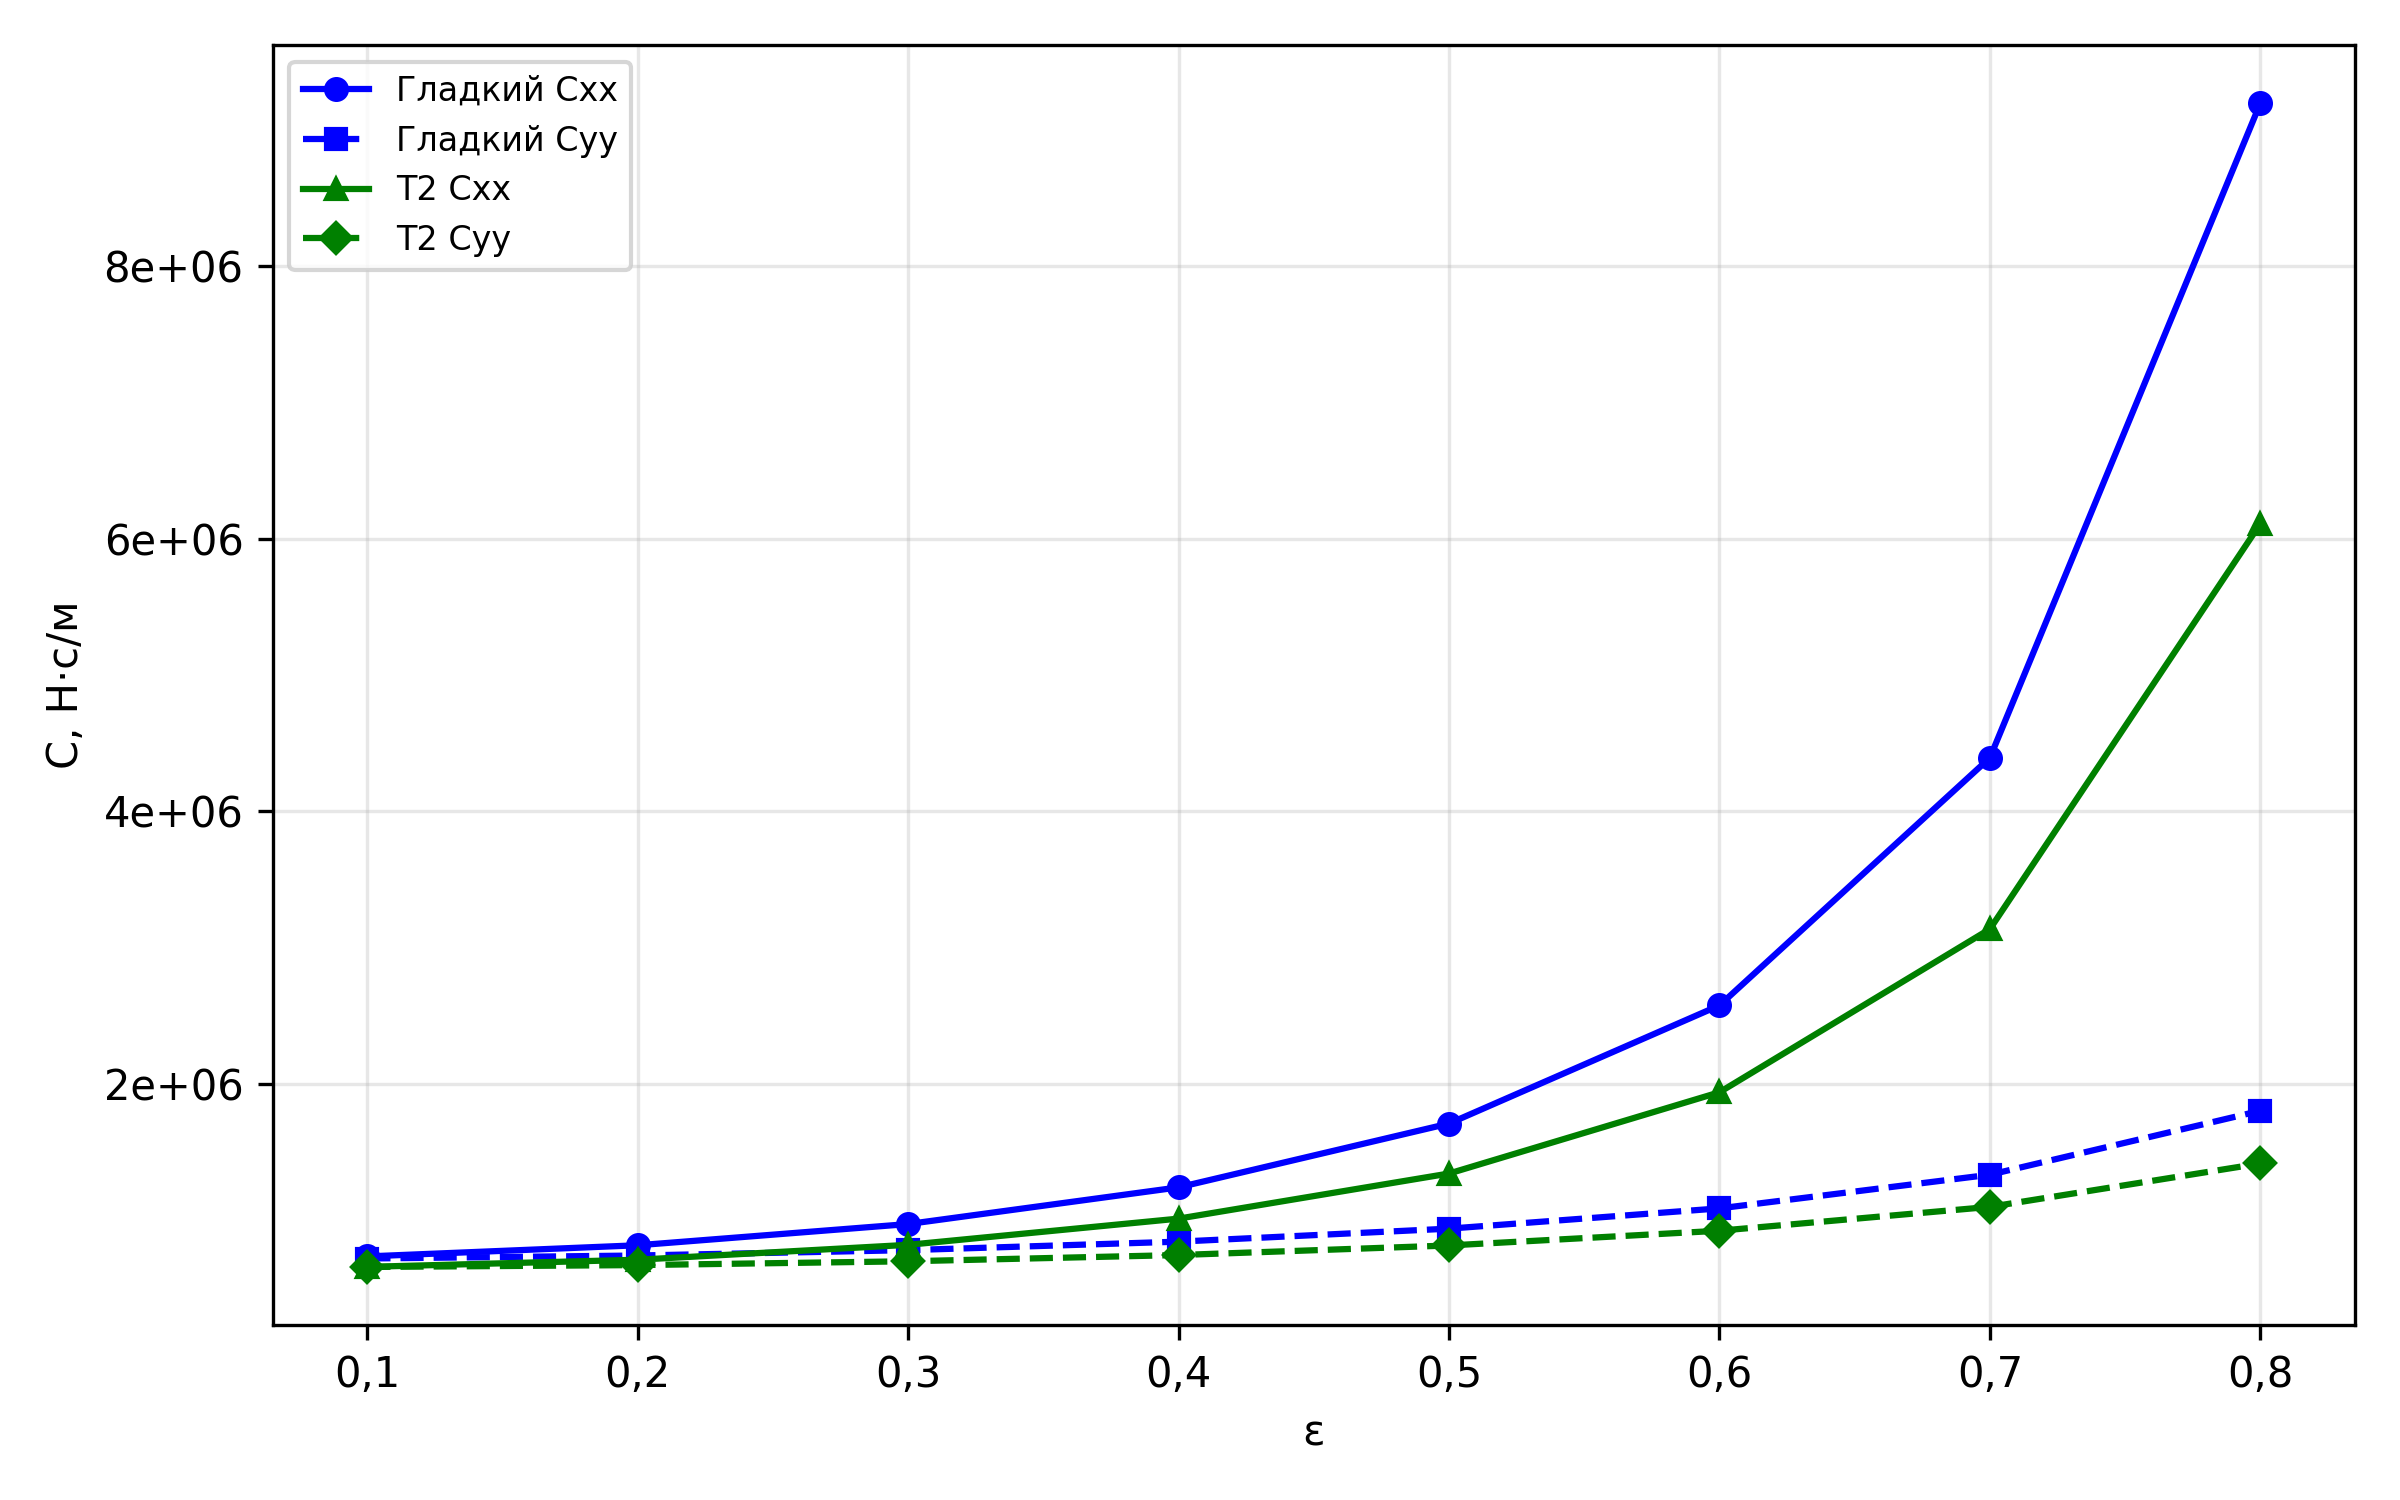
\includegraphics[width=\textwidth,height=0.9\textheight,keepaspectratio]{figures/ch08/fig_8_3.png}
\caption{Зависимость прямых коэффициентов демпфирования $C_{xx}$
  и $C_{yy}$ от эксцентриситета~$\varepsilon$
  для гладкого подшипника и конфигурации~T2.}
\label{fig:dyn_C_direct}
\end{figure}

\begin{figure}[!ht]
\centering
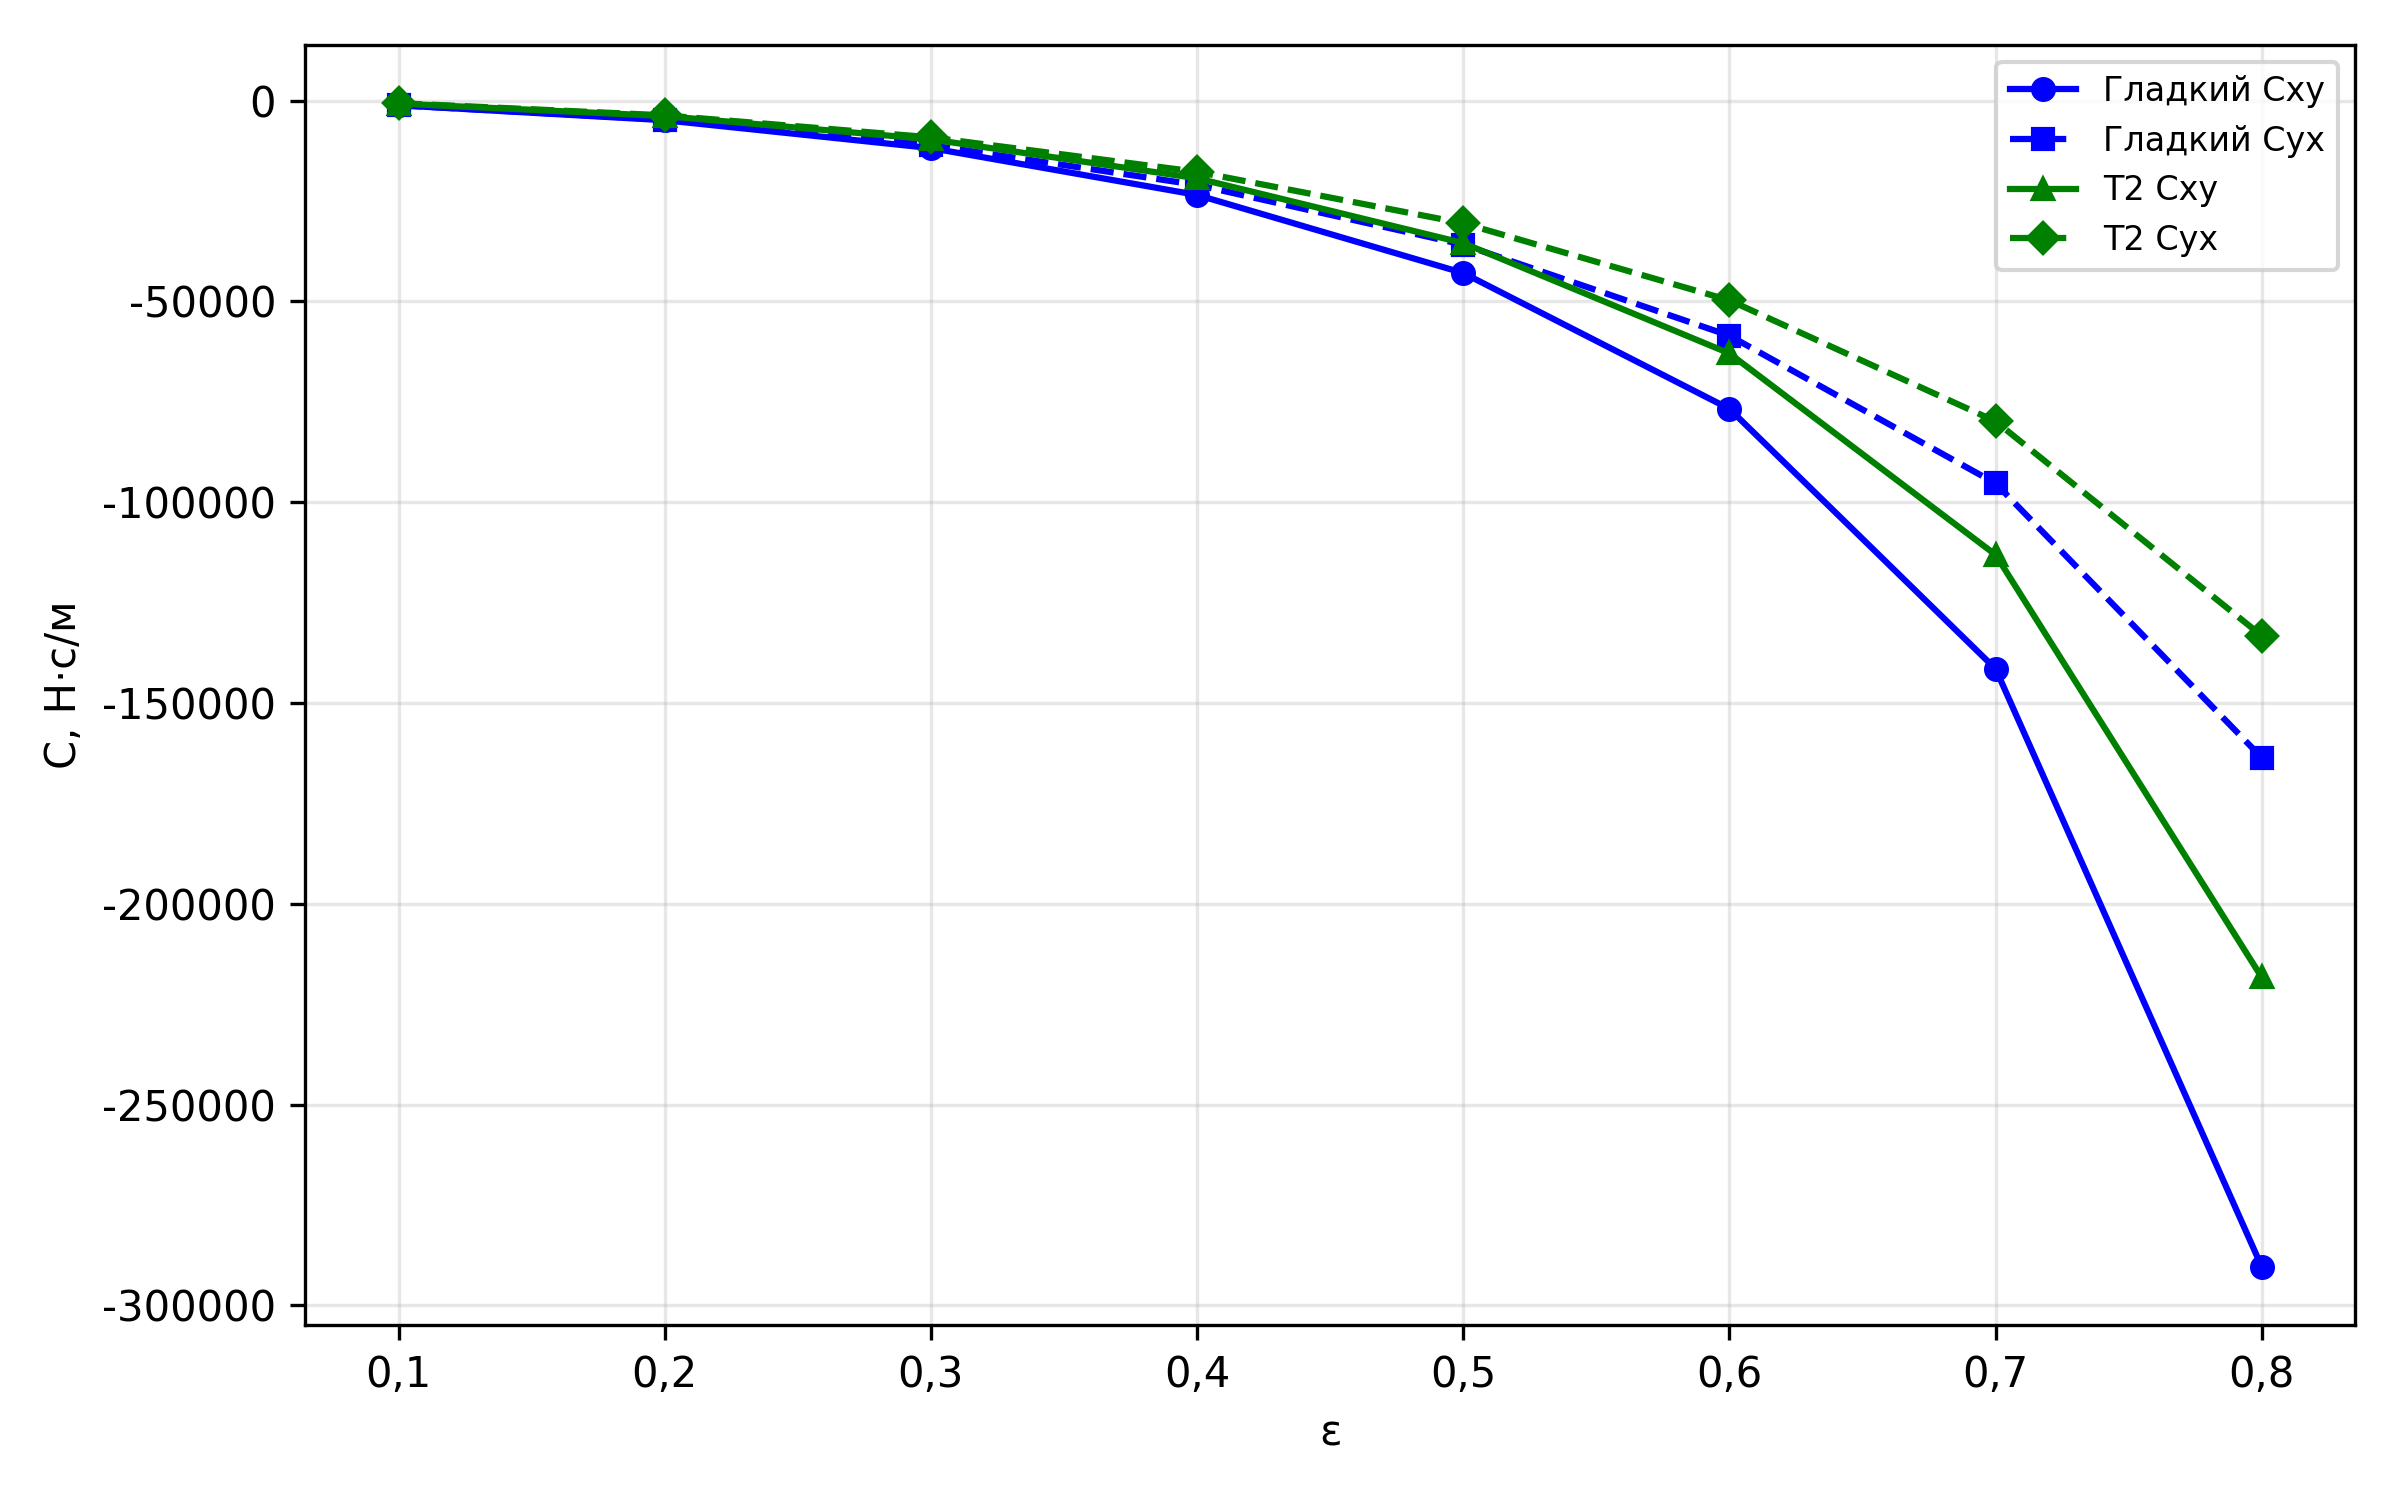
\includegraphics[width=\textwidth,height=0.9\textheight,keepaspectratio]{figures/ch08/fig_8_3a.png}
\caption{Зависимость перекрёстных коэффициентов демпфирования $C_{xy}$
  и $C_{yx}$ от эксцентриситета~$\varepsilon$.}
\label{fig:dyn_C_cross}
\end{figure}

\FloatBarrier


\section{Устойчивость и динамический отклик ротора}

\textit{Устойчивость.}
Во всём исследованном диапазоне
$\varepsilon = 0{,}2$--$0{,}6$ максимальная вещественная часть
собственных значений матрицы состояния
$\mathrm{Re}(\lambda_{\max}) < 0$ для обоих вариантов~--
система линейно устойчива
(рисунок~\ref{fig:dyn_Re_max}). С ростом~$\varepsilon$
значение $\mathrm{Re}(\lambda_{\max})$ становится более
отрицательным, то есть запас устойчивости увеличивается.

Конфигурация~T2 даёт существенно более отрицательные значения
$\mathrm{Re}(\lambda_{\max})$ по сравнению с гладким
подшипником. При $\varepsilon = 0{,}6$:
$\mathrm{Re}(\lambda_{\max})^{(T2)} = -282{,}5$ против
$-122{,}3$ у гладкого. Таким образом, конфигурация~T2 обеспечивает существенно более
высокий запас линейной устойчивости по сравнению с гладким
подшипником.

\begin{figure}[!ht]
\centering
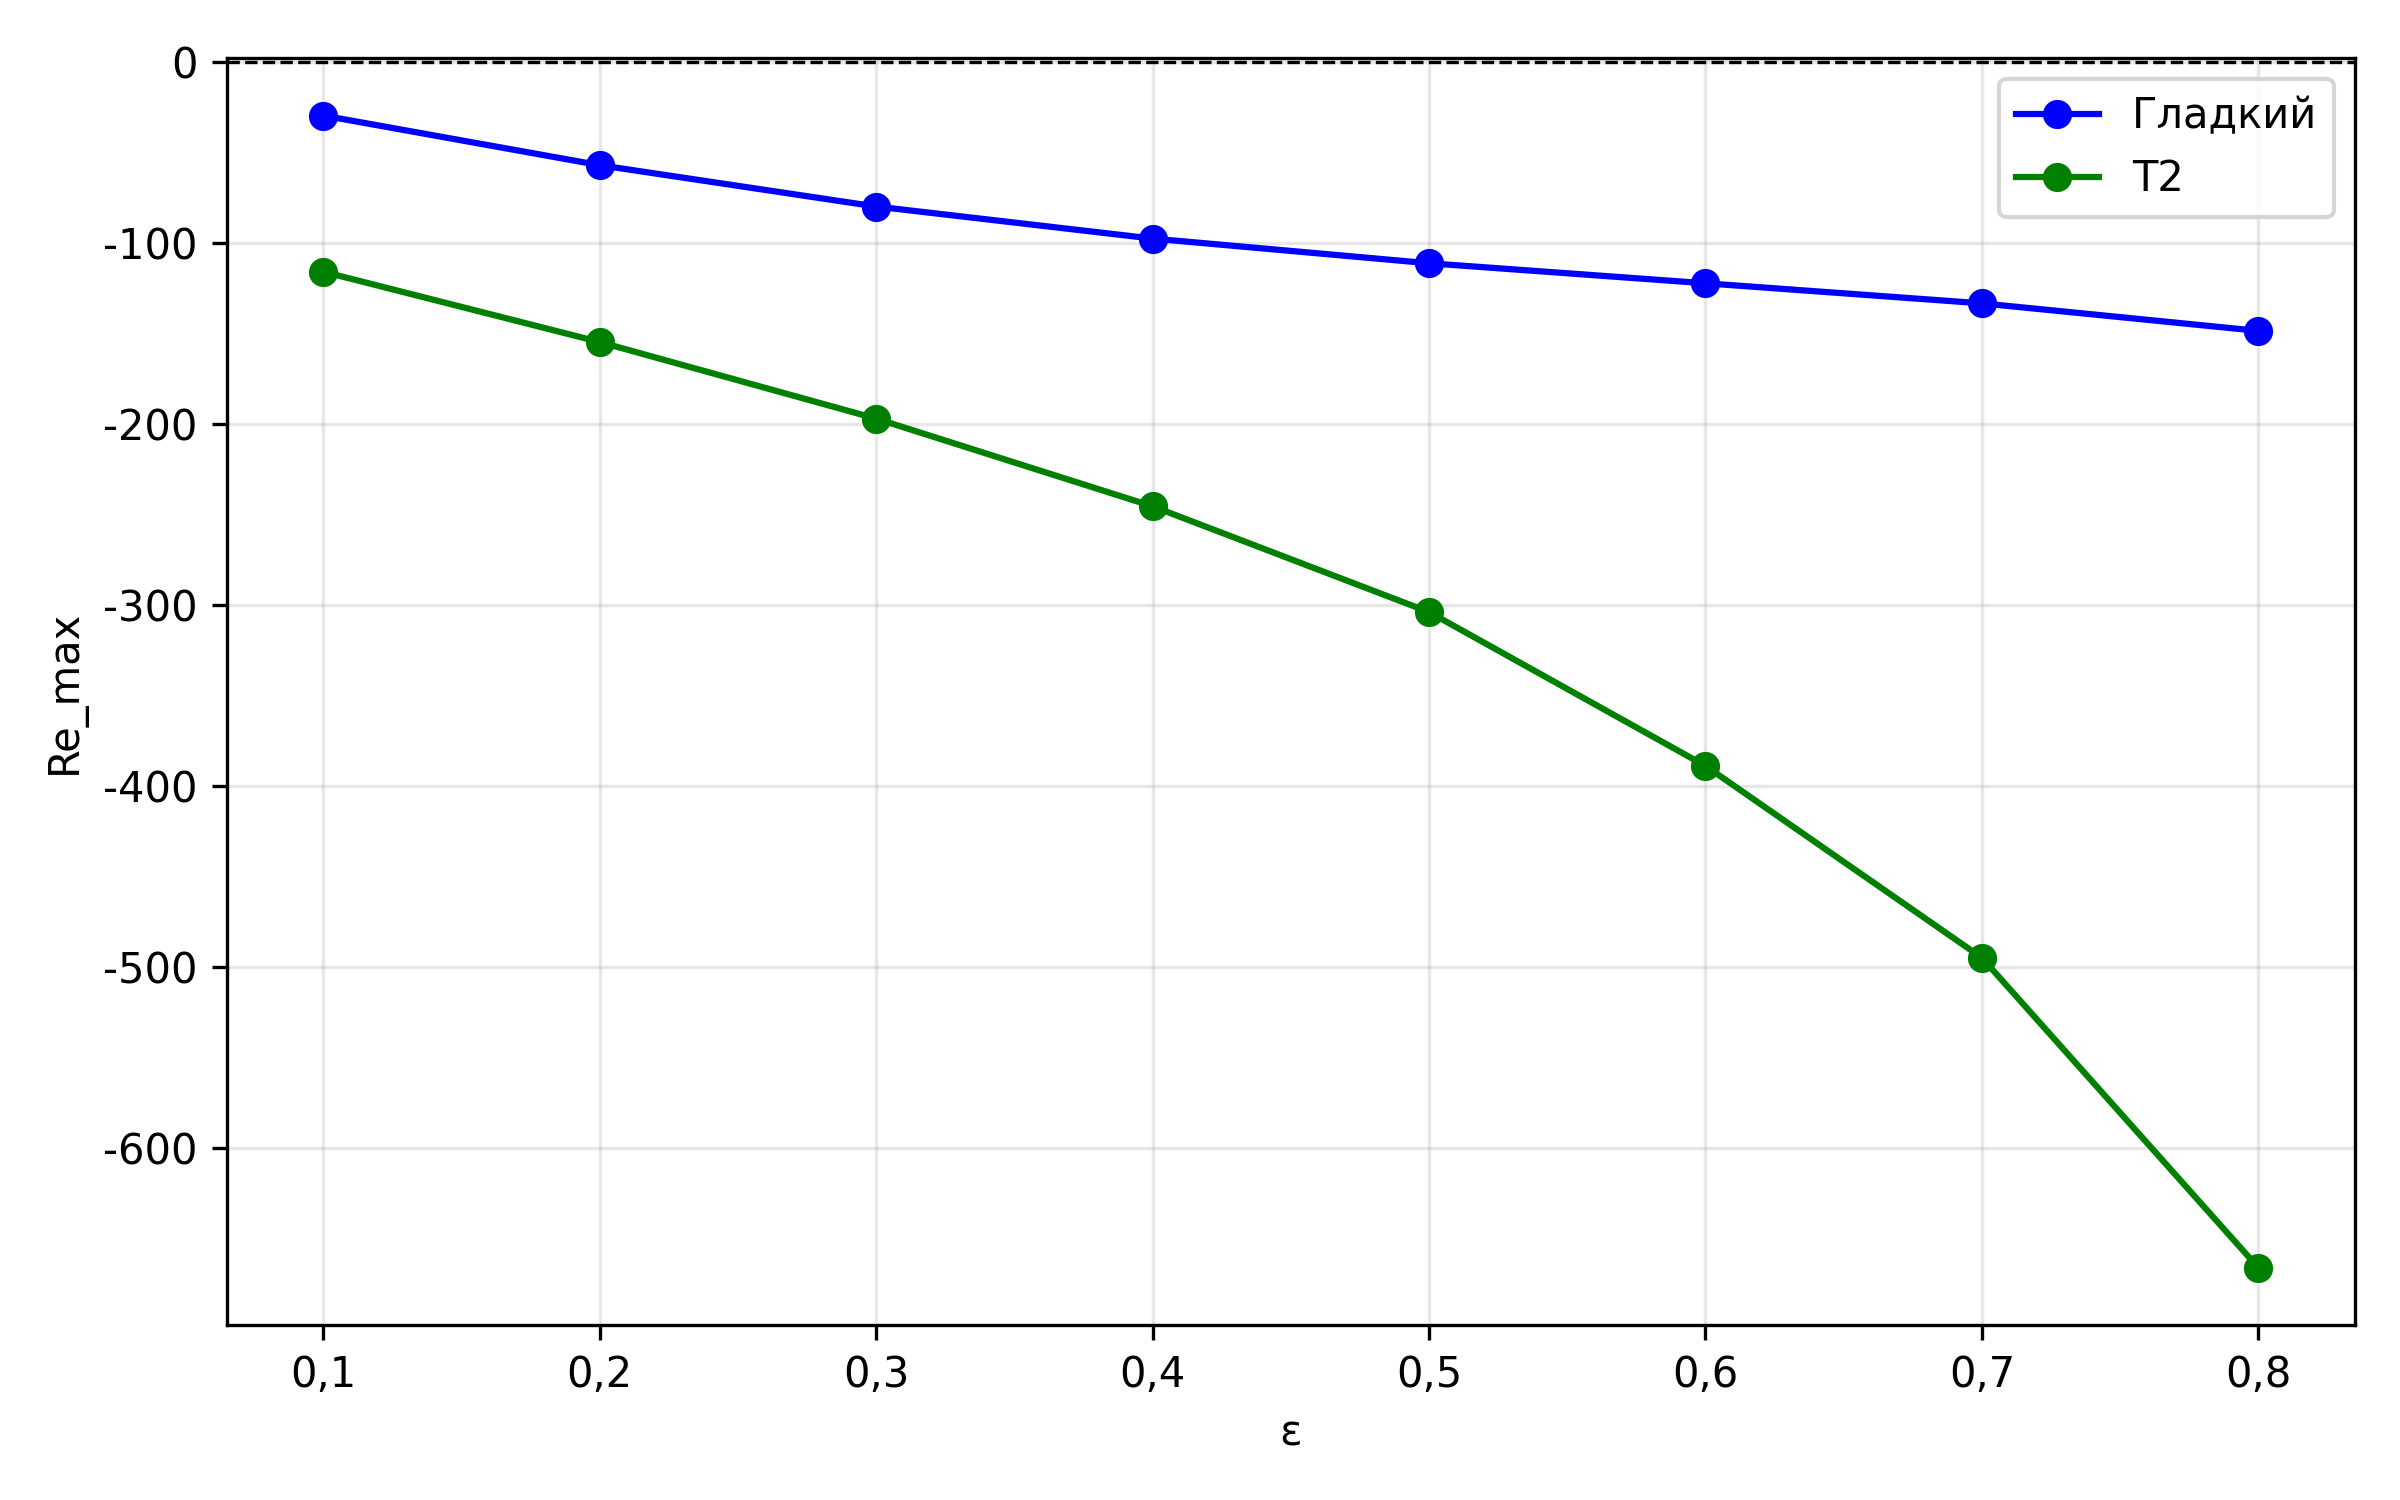
\includegraphics[width=\textwidth,height=0.9\textheight,keepaspectratio]{figures/ch08/fig_8_4.png}
\caption{Зависимость максимальной вещественной части собственных
  значений $\mathrm{Re}(\lambda_{\max})$ от
  эксцентриситета~$\varepsilon$. Пунктирная горизонталь
  $\mathrm{Re} = 0$~-- граница устойчивости.}
\label{fig:dyn_Re_max}
\end{figure}

\FloatBarrier

\textit{Динамический отклик ротора.}
Для $\varepsilon = 0{,}6$ выполнено численное интегрирование
линейной системы~\eqref{eq:dyn_ode_x}--\eqref{eq:dyn_ode_y}
в течение 20~оборотов при начальном возмущении
$\xi_0 = 0{,}01c$. Полная траектория центра цапфы
восстанавливается как $x_{\mathrm{tot}} = x_0 + \xi$,
$y_{\mathrm{tot}} = y_0 + \eta$.

Для гладкого подшипника: $\max|\xi| = 0{,}50$~мкм,
$\max|\eta| = 0{,}22$~мкм. Для~T2: $\max|\xi| = 0{,}50$~мкм,
$\max|\eta| = 0{,}11$~мкм. Максимальные отклонения значительно меньше
радиального зазора $c = 50$~мкм, что подтверждает применимость
линейного приближения. Конфигурация~T2 вдвое уменьшает
поперечную составляющую движения ротора. Временны\'{е} зависимости координат показаны на рис.~\ref{fig:dyn_orbit_time}, а траектории в плоскости $(x, y)$ -- на рис.~\ref{fig:dyn_orbit_xy}.

\begin{figure}[!ht]
\centering
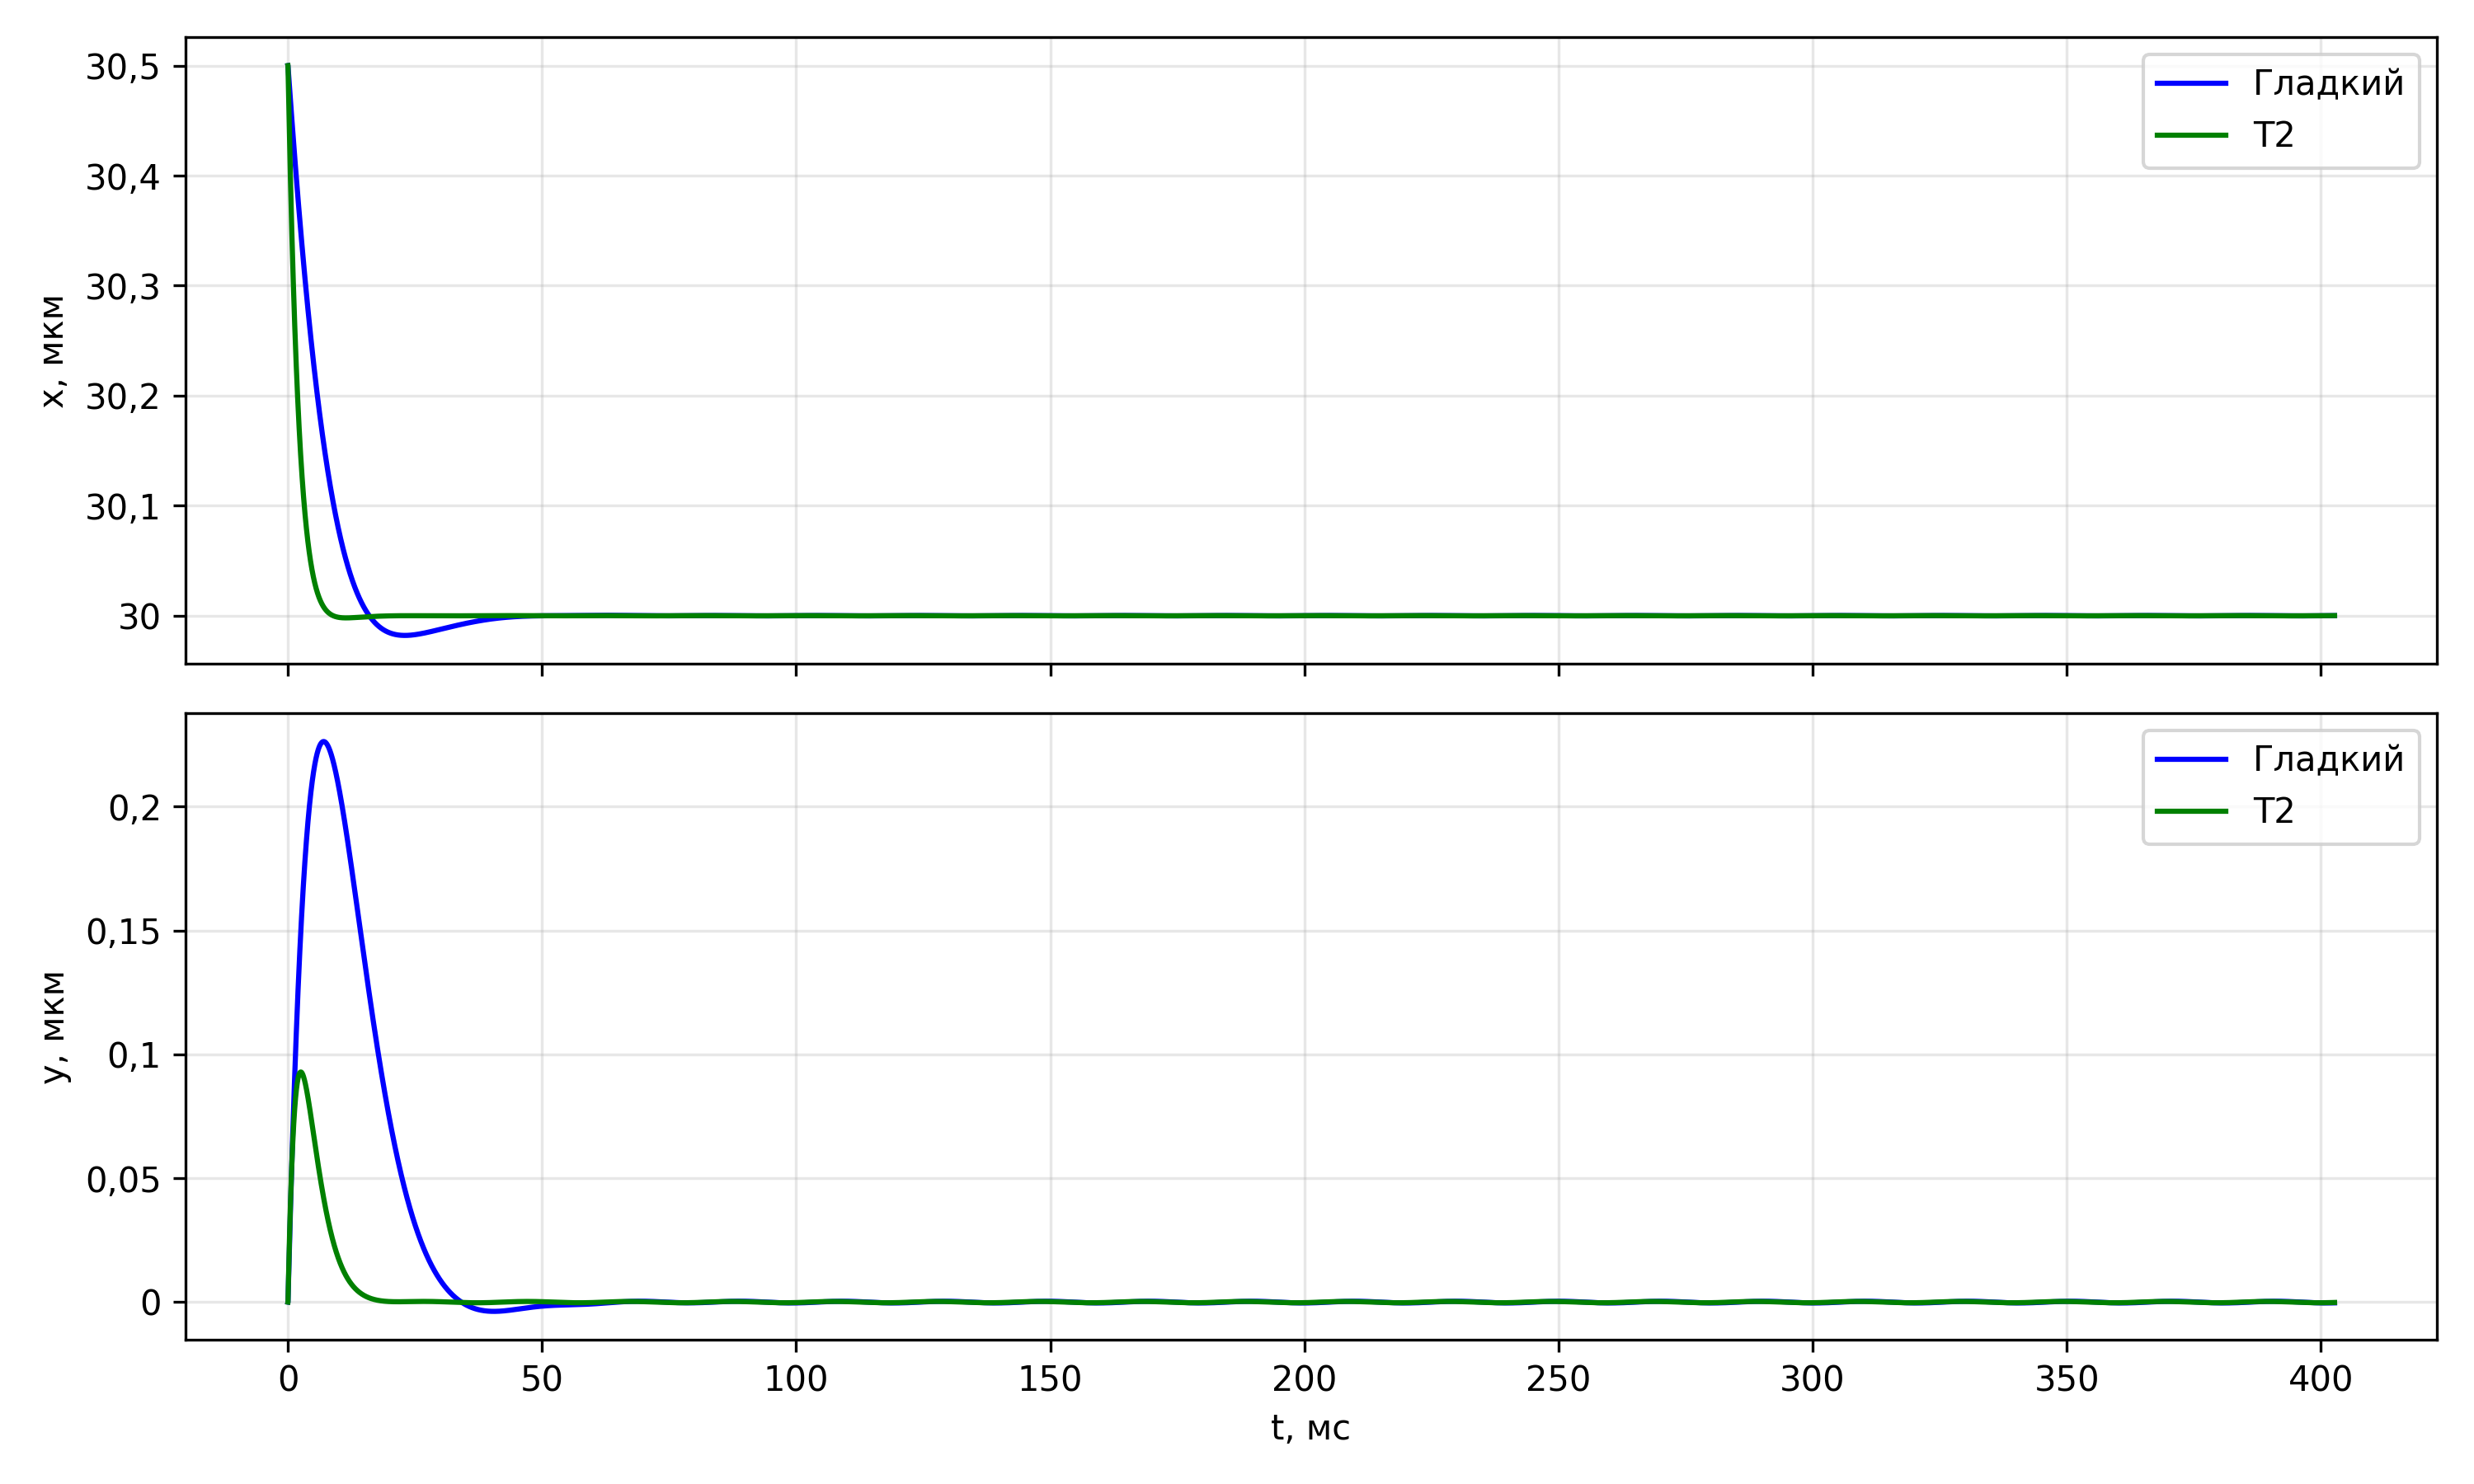
\includegraphics[width=\textwidth,height=0.9\textheight,keepaspectratio]{figures/ch08/fig_8_5.png}
\caption{Временны\'{е} зависимости координат центра цапфы
  $x_{\mathrm{tot}}(t)$ и $y_{\mathrm{tot}}(t)$
  при $\varepsilon = 0{,}6$ для гладкого подшипника
  и конфигурации~T2.}
\label{fig:dyn_orbit_time}
\end{figure}

\begin{figure}[!ht]
\centering
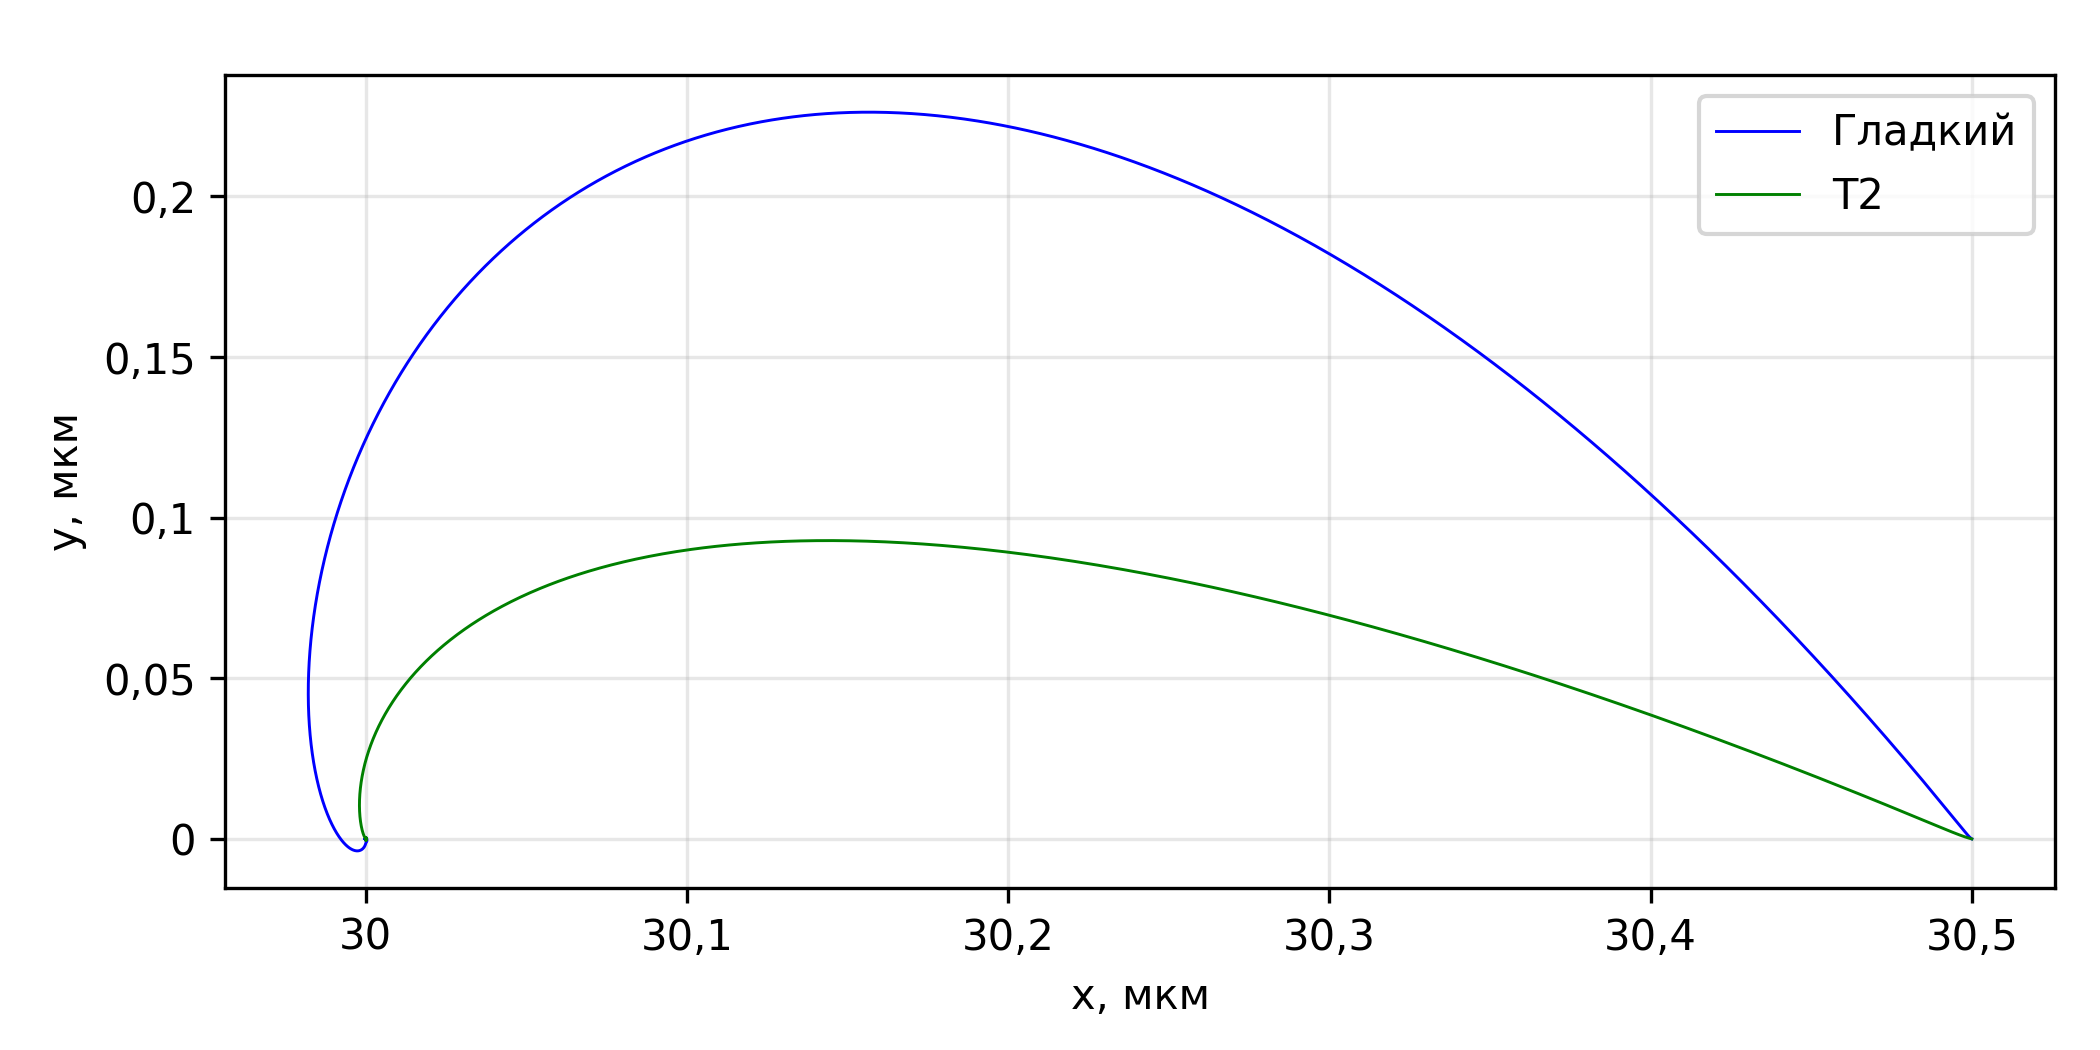
\includegraphics[width=\textwidth,height=0.9\textheight,keepaspectratio]{figures/ch08/fig_8_6.png}
\caption{Траектория центра цапфы в плоскости
  $(x_{\mathrm{tot}},\, y_{\mathrm{tot}})$
  при $\varepsilon = 0{,}6$ для гладкого подшипника
  и конфигурации~T2.}
\label{fig:dyn_orbit_xy}
\end{figure}

\FloatBarrier
\section*{Выводы по главе~8}
\phantomsection\addcontentsline{toc}{section}{Выводы по главе~8}

Разработана линейная динамическая модель системы «ротор~--
подшипник скольжения с микроструктурированной поверхностью»~\cite{han2022,conti2016,cui2018,bashmur2024a,bashmur2024b}.
Модель основана на статическом и динамическом уравнениях
Рейнольдса; динамический член выводится из единой функции
зазора~\eqref{eq:dyn_h} без дополнительных корректирующих
слагаемых. Коэффициенты жёсткости и демпфирования вычислены
методом центральных конечных разностей вокруг одной рабочей
точки.

Проведён сравнительный анализ гладкого подшипника
и конфигурации~T2 в диапазоне
$\varepsilon = 0{,}2$--$0{,}6$. Установлено, что текстура~T2
существенно увеличивает прямые коэффициенты динамической
жёсткости: при $\varepsilon = 0{,}6$ значение $K_{xx}$
возрастает на~$78\,\%$.

Анализ линейной устойчивости по знаку
$\mathrm{Re}(\lambda_{\max})$ показал, что оба варианта
устойчивы во всём исследованном диапазоне эксцентриситетов.
Конфигурация~T2 обеспечивает существенно более высокий запас
линейной устойчивости по сравнению с гладким подшипником.

При $\varepsilon = 0{,}6$ текстурированный вариант примерно вдвое уменьшает максимальное отклонение ротора
по оси~$y$ ($\max|\eta|$:
с $0{,}22$~мкм до $0{,}11$~мкм). Максимальные отклонения ротора значительно
меньше радиального зазора, что подтверждает применимость
линейного приближения.

Перекрёстные коэффициенты демпфирования $C_{xy}$, $C_{yx}$
проявили повышенную чувствительность к шагу численного
дифференцирования и не используются как окончательные
количественные результаты. Верификация прямых жёсткостей
и демпфирований подтвердила их численную устойчивость
при изменении шага и сетки.

Полученные результаты дополняют выводы главы~5 о статических
преимуществах текстурирования, показывая, что применение
детерминированных микроструктур улучшает также динамические
характеристики радиального подшипника скольжения.
